\documentclass{article}
\usepackage[utf8]{inputenc}
\setlength\parindent{2pt}
\usepackage{multirow}
\usepackage{graphicx}
\usepackage{siunitx}
\usepackage{float}
\usepackage{derivative}
\usepackage{amsmath,amssymb}


\title{SURP Computing Project 2020: Lechun Xing \\ CTA200H \\ Supervisor: Jonathan Braden}
\author{Lechung Xing - 1004705170 }
\date{May 8th 2020}

\begin{document}

\maketitle
% Part 1
\section{Clone folder from Github}
git branch:\\ * dev(development branch)\\   master(main branch)
% Part 2
\section{Units}
\subsection{(a) find dimensions of field $\phi$ and potential energy density $V(\phi)$}
Given: $[c]=light speed=LT^{-1}$ and 
$[\hbar]=ML^2{T^{-1}}=[S]$

\vspace{3mm}
Action $S=\int{d^d{x}dt({(\dot{\phi}})^2}/{2c^2}-{(\partial_x{\phi})^2}/2-V(\phi))$

\vspace{3mm}
Replace
$[\dot{\phi}]=[\phi]T^{-1}$ and
$[\partial_x{\phi}]=[\phi]/x=[\phi]x^{-1}$ where [x]=[L]

\vspace{3mm}
Dimension $[S]=L^d{T}({[\phi]^2{T^{-2}}}/L^2{T^{-2}}-[\phi]^2{L^{-2}}-[V(\phi)]$

\vspace{3mm}
Simplify $[S]={L^{d-2}T}({[\phi]^2}-[\phi]^2-L^2[V(\phi)])=[\hbar]=ML^2{T^{-1}}$

\vspace{3mm}
After cancelling the ${[\phi]^2}$ terms and collecting the $L$ terms:

\vspace{3mm}
We derived the dimension of 
$[V(\phi)]=ML^{2-d}T^{-2}$

\vspace{5mm}
Recall PDE: $\frac{1}{c^2}{\frac{\partial^2\phi}{\partial{t^2}}}-{\frac{\partial^2\phi}{\partial{x^2}}}+{\frac{\partial{V}}{\partial{\phi}}}=0$

\vspace{3mm}
The first 2 terms differ only by a constant $A$, they share the same dimension as in the Action expression [S] listed above. Thus, we can rewrite PDE:

\vspace{3mm}
$A[\phi]L^{-2}+[V][\phi]^{-1}=0$ Replace the dimension of [V] and collect $[\phi]$ terms:

\vspace{3mm}
We derived the dimension of 
$[\phi]=(-A)^{-1/2}L[V]^{1/2}=(L^{4-d})^{1/2}M^{1/2}T^{-1}$, in which $d$ is spatial dimensions.

\subsection{(b) introduce scalar $\Lambda, x_0, t_0$, rewrite action S}

Given: $\phi=\Lambda{\bar{\phi}}$ and $x=x_0{\bar{x}}$ and $t=t_o{\bar{t}}$

\vspace{3mm}
Derive: $\dot{\phi}=\Lambda{\dot{\bar\phi}}=\Lambda{\partial_t}{\bar\phi}$ and $\partial_x{\phi}=\frac{\partial\phi}{\partial{x}}=\frac{\partial\phi}{\partial}{{(x_0\bar{x})}}=\frac{1}{x_0}{\partial_\bar{x}}{(\Lambda{\bar\phi})}=\frac{\Lambda}{x_0}{\partial_\bar{x}}{\bar\phi}$

\vspace{3mm}
Similarly convert the differentials: $dx=x_0{d\bar{x}}$ and $dt=t_0{d\bar{t}}$

\vspace{3mm}
Action $S=\int{{x_0}^d{(d\bar{x}})^d{(t_0{d\bar{t}})}[\frac{\Lambda^2{\dot{\bar{\phi}}}^2}{2c^2}-\frac{1}{2}{(\frac{\Lambda}{x_0})^2(\partial_{\bar{x}}{\bar\phi}})^2-V(\Lambda\bar\phi)]}$

\subsection{(c) rewrite PDE in terms of  derivatives of $\bar{t}, \bar{x}$}
Substitute 3 scalars into PDE: $\frac{1}{c^2}{\frac{\partial^2}{\partial{t^2}}(\Lambda\bar\phi)}-\frac{\partial^2}{\partial{x^2}}(\Lambda\bar\phi)+\frac{\partial{V}}{\partial(\Lambda\bar\phi)}=0$

\vspace{3mm}
Pull out $\Lambda$: $\frac{\Lambda}{{c^2}{t_0}^2}{{\partial^2}_{\bar{t}}\bar\phi}-{\frac{\Lambda}{{x_0}^2}{\partial^2_{\bar{x}}}}{\bar\phi}+{\frac{\partial{V(\bar\phi)}}{\partial{\bar\phi}}}=0$


%Which code file? Which eqn?
\subsection{(d) rewrite dimensionless eqn. in the code for  $\hbar=c=1$}
For $\hbar=c=1$: 
$\frac{\Lambda}{{t_0}^2}{{\partial^2}_{\bar{t}}\bar\phi}-{\frac{\Lambda}{{x_0}^2}{\partial^2_{\bar{x}}}}{\bar\phi}+{\frac{\partial{V}}{\partial{\bar\phi}}}=0$ all expressed in terms of scaling factors or dimensionless quantities.

%Part 3
\section{Plot field evolution $\phi(x, t)$}
\begin{figure}[H]
    \centering
    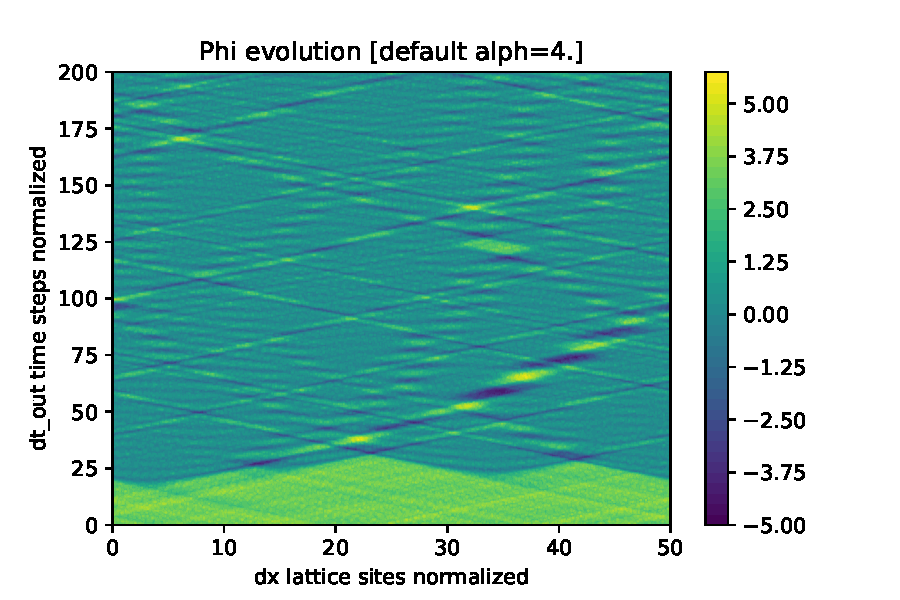
\includegraphics[scale=0.7]{Phi_evo_default.pdf}
    \caption{Field evolution $\phi(t, x)$ plotted from $<fields.dat>$ with the normalized lattice sites $x\in{[0, 1024*dx]}$ and the normalized time steps $t\in{[0, 200]}$.}
    \label{fig:Q3}
\end{figure}

$\phi(t, x)$ values drop across all 1024 lattice sites as t increases. The slanted bands extending over Fig.1 indicate the fluctuations of $\phi(t, x)$ values among the overall decreasing trend for larger t.

% Part 4
\section{Energy conservation}

\begin{figure}[H]
    \centering
    \includegraphics[scale=0.7]{E_dev_alph=4}
    \caption{Violation of Energy conservation vs. output time steps $dt_{out}$. Blue data is calculated from $<fields.dat>$ according to $E=\sum_i(\frac{1}{2}{\dot\phi_i}^2+\frac{1}{2}{(\nabla{\phi})^2}_i+V(\phi_i))$, $i$ means summation over 1024 lattice sites. Red dashed line is the power fitting model $E = a*{t}^b$, a, b are parameters. $t=dt'$ array, determined by $\alpha=dx/dt$ in $<evolve-scalar.f90>$}
    \label{fig:Q4}
\end{figure}

The size of Energy deviation $|E(t) - E(0)|$ seems to increases linearly with t. When $\alpha = 0.95$ or any value smaller than 1., the code does not output data file. 

% Part 5
\section{Energy violation: adjust $\alpha$}



\begin{figure}[H]
    \centering
    \includegraphics[scale=0.7]{E_dev_alph_all}
    \includegraphics[scale=0.7]{E_dev_alph_all_log}
    \caption{Combined $|E(t) - E(0)|$ plot for 6 $\alpha$ values. The bottom plot is with log y axis.}
    \label{fig:Q5}
\end{figure}

Fig.3 shows $|E(t) - E(0)|$ decreases as $\alpha$ increases from 1. to 32..
b = 1 if rounded to the nearest integer except for the $\alpha=32$ plot. However, today I realized this part is asking for how Energy conservation error is scaled with dt' instead of the time evolution of $E(t) - E(0)$. I noticed from Fig.3.(log scale) that for each dt', the Error size satisfies $\frac{Error[i]}{Error[j]}\propto{\frac{dt'[i]}{dt'[j]}}^{b}$, where i,j are indices from dt' array. Averaging over the 6 b values, I conclude $b\approx9$. This is the answer for Part 6. 

\begin{figure}[H]
    \centering
    \includegraphics[scale=0.35]{E_dev_alph=1}
    \includegraphics[scale=0.35]{E_dev_alph=2}
    \includegraphics[scale=0.35]{E_dev_alph=4}
    \includegraphics[scale=0.35]{E_dev_alph=8}
    \includegraphics[scale=0.35]{E_dev_alph=16}
    \includegraphics[scale=0.35]{E_dev_alph=32}
    \caption{Power fit for different $\alpha$ curves as in Fig.3.}
    \label{fig:Q1}
\end{figure}

$\alpha=1., a =  10.603, b =  0.928$ with the variance in a and b to be 0.064 and 0.001, respectively. $\alpha=2., a = 0.019, b =  1.011$ with variance 2.408e-05 and 0.0003. $\alpha=4., a = 3.807e-05, b =  1.011$ with variance, 4.926e-08 and 0.0003. $\alpha=8., a = 7.518e-08, b =  1.011$ with variance, 9.774e-11 and 0.0003. $\alpha=16., a = 1.491e-10, b =  1.010$ with variance 1.927e-13 and 0.0003. $\alpha=32., a = 4.536e-12, b =  0.440$ with variance 9.780e-13 and 0.045. 

\vspace{3mm}
Above fitting are irrelevant to this part. Please see Part 5 instead.



\section{Field evolution: adjust $\lambda$ the shape of $V(\phi)$}

\begin{figure}[H]
    \centering
    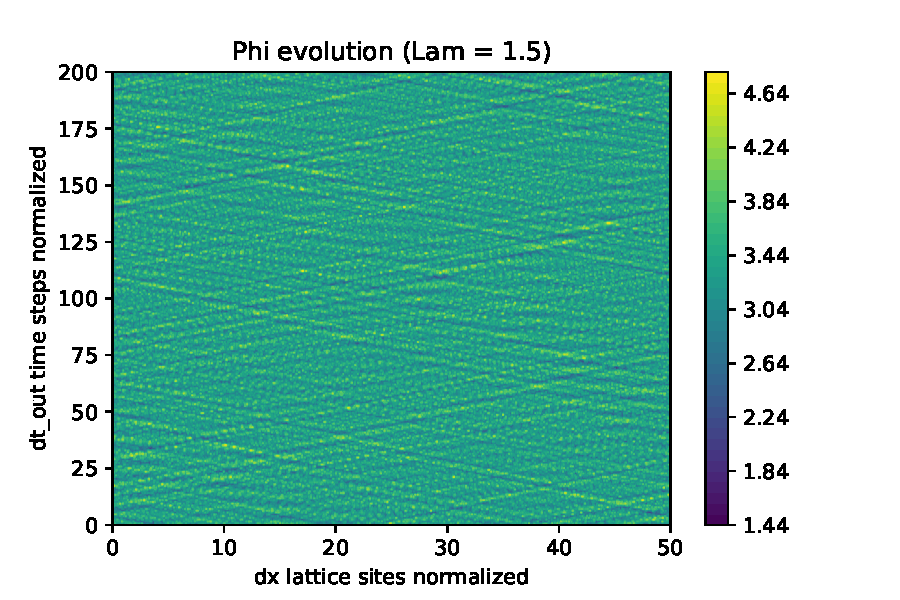
\includegraphics[scale=0.7]{Phi_evo_L1point5}
    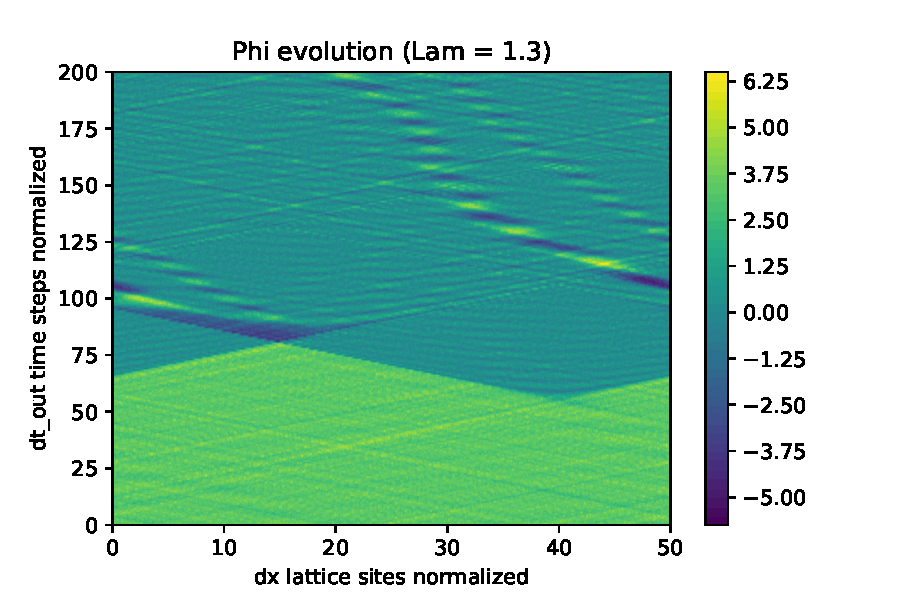
\includegraphics[scale=0.7]{Phi_evo_L1point3}
    \caption{$\lambda=1.5 and 1.3$}
    \label{fig:Q1}
\end{figure}

\begin{figure}[H]
    \centering
    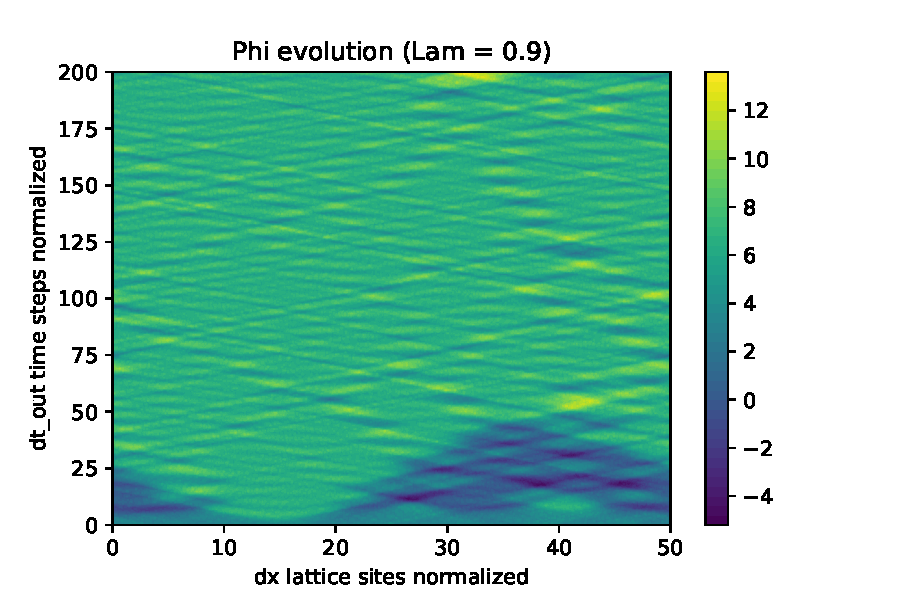
\includegraphics[scale=0.7]{Phi_evo_Lpoint9}
    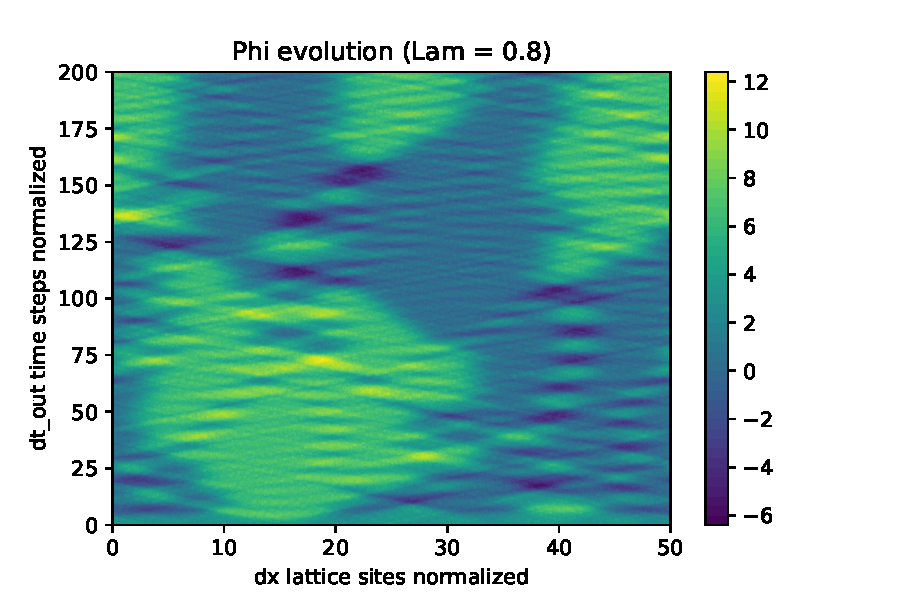
\includegraphics[scale=0.7]{Phi_evo_Lpoint8}
    \caption{$\lambda=0.9 and 0.8$}
    \label{fig:Q1}
\end{figure}

\begin{figure}[H]
    \centering
    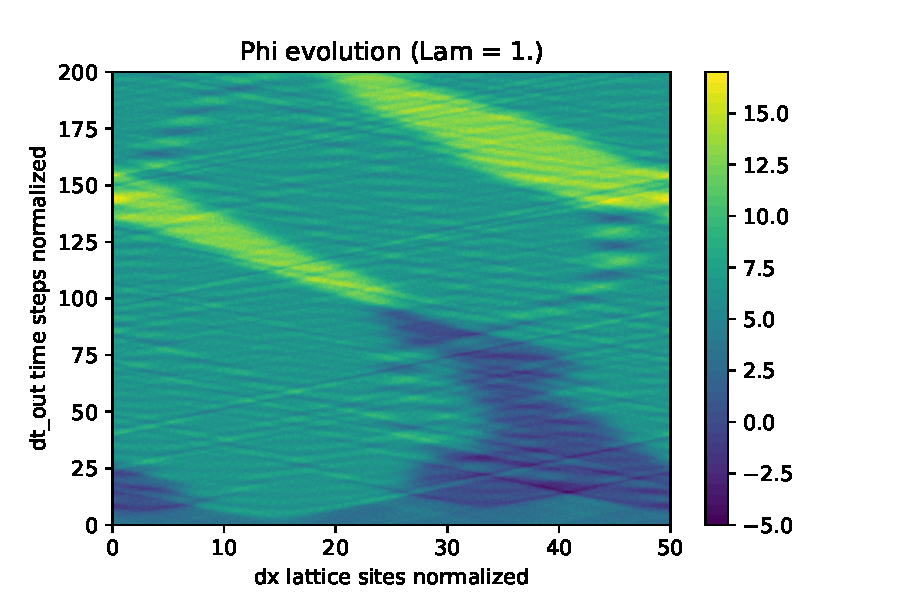
\includegraphics[scale=0.7]{Phi_evo_L1}
    \caption{$\lambda=1.$}
    \label{fig:Q1}
\end{figure}

When $\lambda$ is far away from $1.2$, I no longer see the clear cut (wall) between True vacuum and the False vacuum. especially when $\lambda=1.5>1.2$, field evolves to a stage filled with fluctuations.
\section{Field evolution: adjust initial conditions}

\begin{figure}[H]
    \centering
    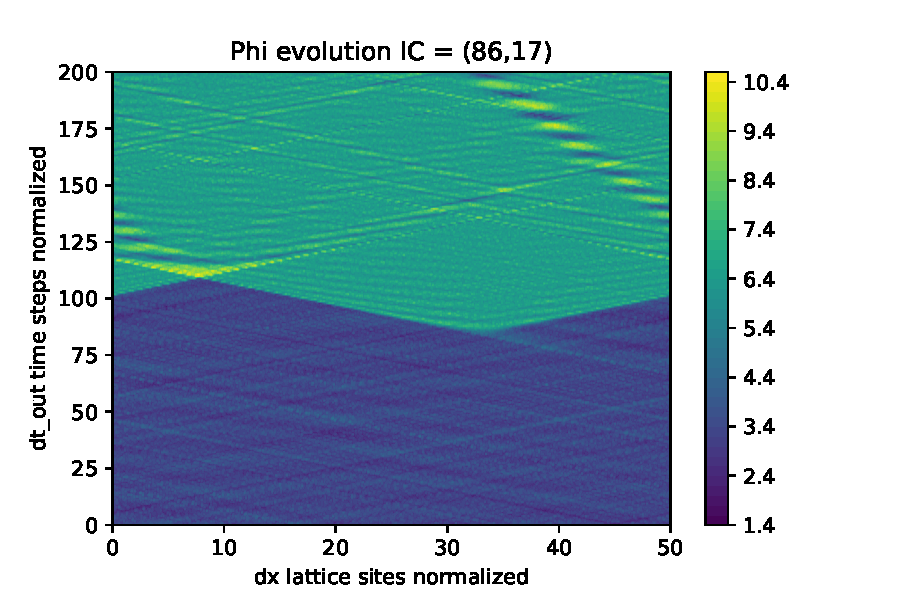
\includegraphics[scale=0.7]{Phi_evo_8617}
    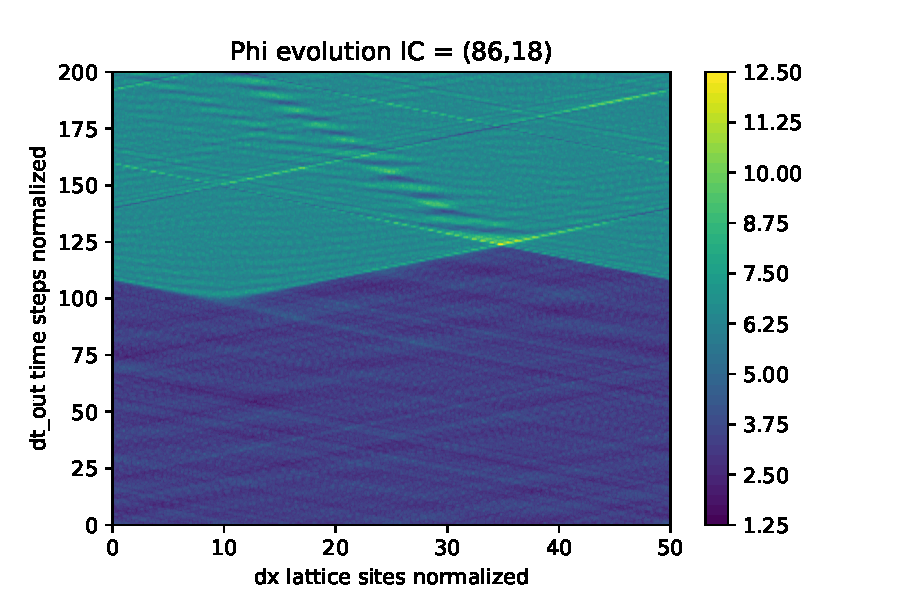
\includegraphics[scale=0.7]{Phi_evo_8618}
    \caption{(86, 17), (86,18) initial conditions}
    \label{fig:Q1}
\end{figure}


\begin{figure}[H]
    \centering
    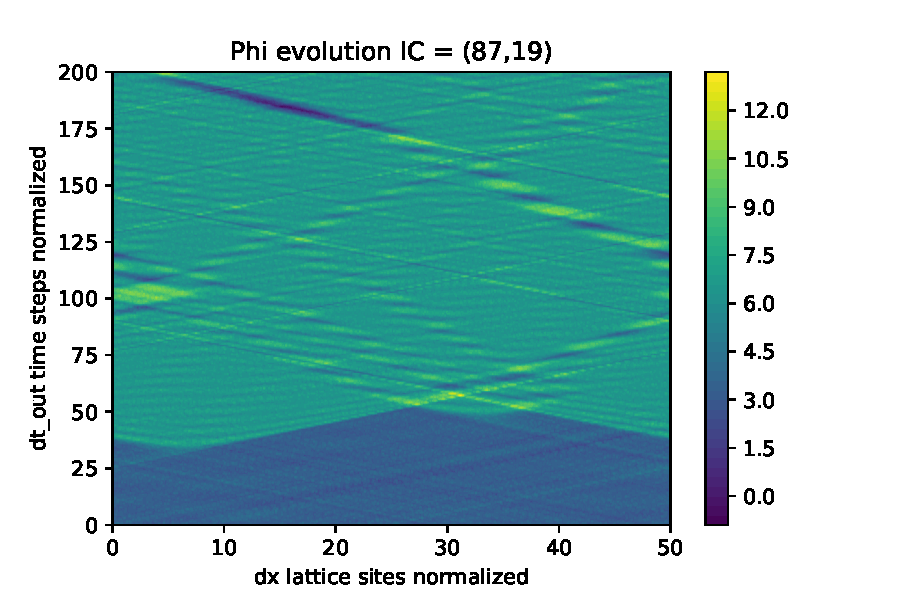
\includegraphics[scale=0.7]{Phi_evo_8719}
    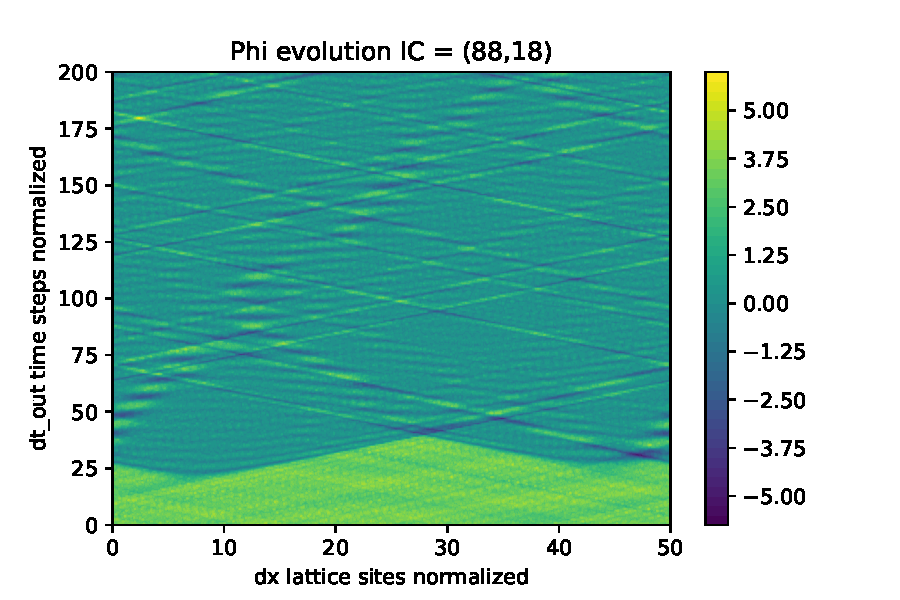
\includegraphics[scale=0.7]{Phi_evo_8818}
    \caption{(87, 19), (88,18) initial conditions}
    \label{fig:Q1}
\end{figure}

\begin{figure}[H]
    \centering
    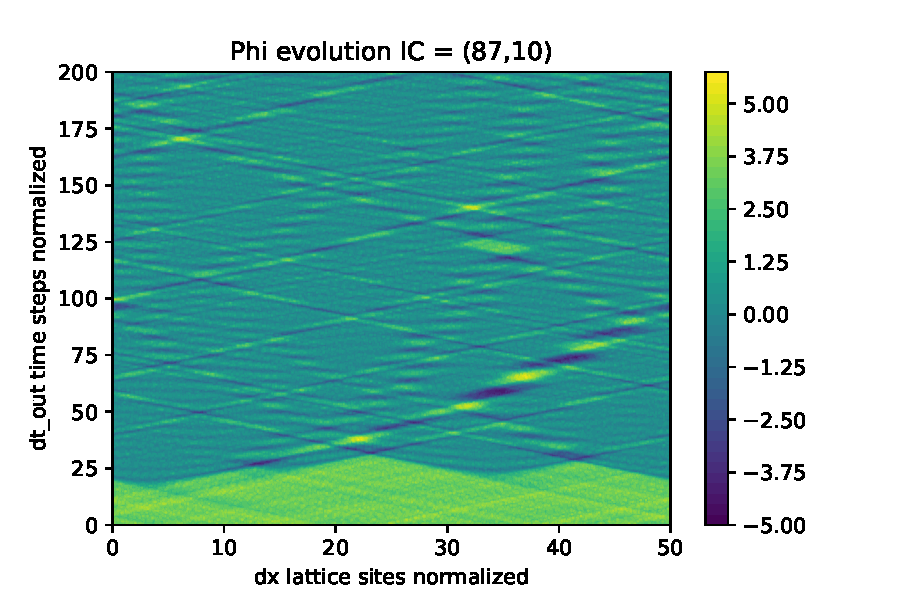
\includegraphics[scale=0.7]{Phi_evo_8710}
    \caption{(87,10) initial conditions}
    \label{fig:Q1}
\end{figure}

For random seeds close to the default (87, 18), the field evolution does not change much in terms of the $\phi$ value difference above and below the wall.
\end{document}